%----------------------------------------------------------------------------------------
%	Background
%----------------------------------------------------------------------------------------
\todo{
- FPGA diagram
- CPU-CFU functional diagram

- Spectogram
- Another modulation
- CFU playgroud videos take CFU block scheme 

}

\chapter{Background} \label{Chapter 2}

\section{Signal modulation}

Signal modulation is a process of modifying a signal to enable it to carry information from one point to another. In wireless communication systems, modulation encodes information onto a carrier wave transmitted over electromagnetic waves. Signal modulation includes manipulating a carrier signal by a modulating signal to produce a modulated signal that contains the desired information. The carrier signal is typically a high-frequency sine wave. The modulating signal is the signal that contains the information that needs to be transmitted. The modulated signal is then transmitted to the receiver, which is demodulated to extract the original modulating signal. The main reasons for modulation are bandwidth utilization, noise, interference mitigation, and efficient signal propagation~\cite{communication_systems_engineering}.

Generally, frequency modulation can be divided into analog and digital. The name describes the nature of the data transmitted. The most common types of analog modulation used in wireless communication systems are Amplitude Modulation (AM), Frequency Modulation (FM), and Phase Modulation (PM)~\cite{fundamentals_or_wireless}. Some of the popular digital modulation techniques include Amplitude Shift Keying (ASK), Frequency Shift Keying (FSK), Phase Shift Keying (PSK), and Quadrature Amplitude Modulation (QAM)~\cite{communication_systems_engineering,analog_digital_overview}. These modulation techniques vary in terms of the number of bits they can transmit per symbol, spectral efficiency, and susceptibility to noise and interference. They are widely used in various communication systems, including radio and television broadcasting, cellular networks, and satellite communication systems.

Example of digital modulation Amplitude Shift Keying -- when carrier signal amplitude encodes transmitted digital signal is depicted in Figure~\ref{fig:ask}.

\begin{figure}[t]
\centering
\caption{Amplitude Shift Keying (ASK) visualization~\cite{pysdr} }
% 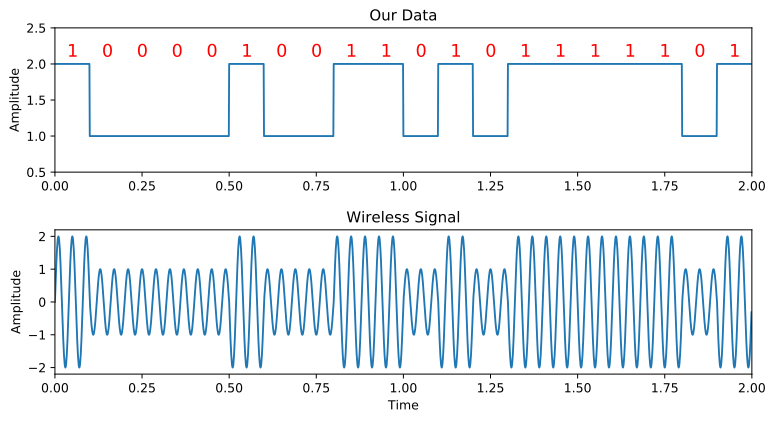
\includegraphics[width=0.9\textwidth]{ask.png}
\includesvg[width=0.9\textwidth]{graphic/ASK.svg}
\label{fig:ask}
\end{figure}

\section{Signal modulation classification}

Signal modulation classification or Automatic Modulation Recognition (AMR) is the process of identifying the modulation technique used to transmit a signal. Accurately identifying the modulation scheme used in a communication signal is essential for designing effective communication systems, as different modulation techniques require different receiver configurations and signal processing algorithms. Some of AMR applications are:



\begin{itemize}
    \item Cognitive Radio~\cite{cognitive_radio_amr}: Cognitive radio systems aim to dynamically allocate available spectrum to different users based on real-time conditions. AMR plays a crucial role in cognitive radio by enabling the radios to identify and adapt to the modulation schemes used by primary users. This allows users to utilize the spectrum efficiently for better avoidance of interference with other primary users.
    \item Wireless Network Planning: When planning and deploying wireless networks, AMR assists in identifying the modulation schemes employed by neighboring networks. This information is valuable for selecting appropriate frequency channels, optimizing signal parameters, and minimizing interference between neighboring networks.
    \item Electronic Warfare~\cite{amr_warfare}: In military applications, AMR is utilized in electronic warfare to automatically identify and classify enemy communication signals. By recognizing the modulation schemes, military personnel can assess the capabilities, intentions, and threat levels of adversaries and develop appropriate countermeasures.
\end{itemize}



% In wireless communication systems, AMR is used for monitoring and analysis purposes.
% Moreover, signal modulation classification is important for detecting and mitigating interference and jamming in communication systems and ensuring reliable and efficient communication in various applications, such as military, healthcare, transportation, and industrial control systems. \todo{Some reference here}

\subsection{Model input}

% As overviewed in~\cite{amr_deep_networks_overview}, there are different 
There are different approaches to data preparation as the input to the model. Some of them are presented in~\cite{amr_deep_networks_overview}. For example, constellation maps can be used as 2-dimensional input to convolutional neural network~\cite{amr_survey_deep_learning,vgg_simc,learning_constellation_map}. Time-frequency diagram, Eye-diagram, and Amplitude Histogram are also used as preprocessed input to the model~\cite{amr_deep_networks_overview}. A constellation map refers to a graphical representation (xy plane) that depicts the relationship between the different symbols or signal points used in a modulation scheme, like real and complex parts in in-phase and quadrature (IQ) representation of signal, or phase in PSK, as shown in Fig.~\ref{fig:8-psk-constellation}. 



% TODO: didn't find good image for PAM4
% maybe this? https://www.sony-semicon.com/en/technology/laser-diode/optical-vcsel.html 
% or this?    https://en.wikipedia.org/wiki/Eye_pattern#/media/File:Eye_diagram.png

% An eye diagram is a graphical representation of a signal's waveform in digital communication systems. It provides a visual depiction of the signal's amplitude and timing characteristics over multiple periods. To construct an eye diagram, a series of signal waveforms are overlaid and superimposed onto each other, with each waveform corresponding to a single bit or symbol interval. The vertical axis represents the signal amplitude, while the horizontal axis represents time. Eye-diagram for PAM-4 modulation is depicted in Figure~\ref{}


\subsection{Classical approaches}

Over the years, various methods have been proposed for signal modulation classification, ranging from traditional statistical methods to modern machine learning-based approaches. Some of the popular classical classification methods include Linear Discriminant Analysis (LDA)~\cite{LDA_for_simc}
% Quadratic Discriminant Analysis (QDA)~\cite{QDA_for_simc}
, Singular Value Decomposition (SVD)~\cite{svd_af_for_simc},  Maximum Likelihood~\cite{ML_for_simc}, Support Vector Machines (SVMs)~\cite{SVM_for_simc} and XGBoost~\cite{radioml_2018}. 

\subsection{Deep Learning solutions}


\begin{wrapfigure}{r}{0.4\textwidth}
\centering
\caption{Constellation map of 8-PSK: each symbol is encoded as a different phase shift of the carrier sine wave: 0°, 45°, 90°, 135°, 180°, 225°, 270°, 315°, Credit: Wikipedia~\cite{constelation_img}. }
% 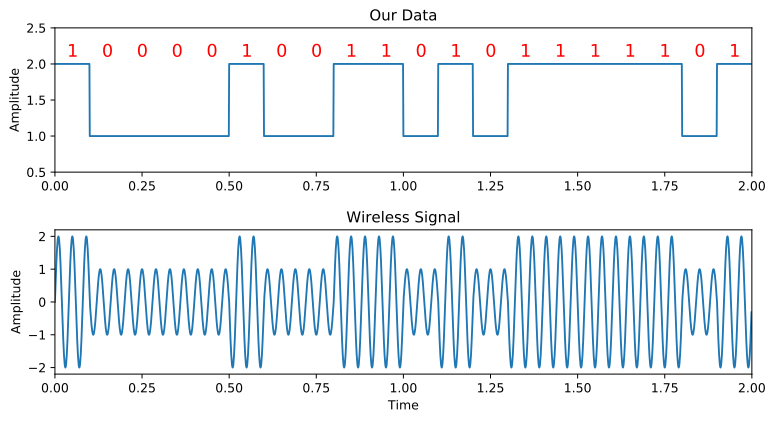
\includegraphics[width=0.9\textwidth]{ask.png}
\includesvg[width=0.38\textwidth]{graphic/8PSK_Gray_Coded.svg}
\label{fig:8-psk-constellation}
\end{wrapfigure}

Usually, transmission data in real life is subject to various sources of distortion, like fading, interference, timing drift due to clock offset, and general noise of the environment. Deep learning models can perform well with much noise if trained properly with high-quality data. %\todo{word for a model that performs well}. - Not sure what that todo means :)

In recent years, Convolutional Neural Networks (CNNs) have emerged as a powerful tool for signal modulation classification. CNNs have shown remarkable performance in various machine-learning tasks, including image recognition, natural language processing, and speech recognition~\cite{cnn_overview}. CNNs have also been applied to signal modulation classification and have achieved good performance, even in noisy and complex environments. As shown in~\cite{radioml_2018,vgg_simc}, they can outperform classical approaches.

As shown in~\cite{vgg_simc}, popular CNN models, like VGG-16~\cite{vgg16} and AlexNet~\cite{alexnet}, perform well on modulation classification. They convert the received data to a constellation image. Another approach is to use an IQ representation of the received data as input for the regular CNN model, which combines convolutional layers, pooling layers, and fully connected layers to extract features from the input signal and classify it into one of the modulation classes. Timothy J O'Shea et al.~\cite{cnn_dnn_simc} show that such models can perform well and outperform classical approaches. Also, they show that the CNN has noticeably higher accuracy than Deep Neural Network (DNN) model. Xiaoyu Liu et al.~\cite{cnn_resnet_cldnn} demonstrated that increasing the depth of the model and using ResNet~\cite{resnet} doesn't improve accuracy much, and Convolutional Long Short-term Deep Neural Network (CLDNN) has a better classification accuracy score. 

Transformer models are a deep learning architecture primarily used for natural language processing (NLP) tasks, such as language translation and text generation~\cite{transformer_nlp_applications}. Unlike traditional recurrent neural networks (RNNs), which process input sequences sequentially, transformers use a self-attention mechanism to process input sequences in parallel, allowing them to capture long-term dependencies more effectively. Recent studies show that transformers perform well on other tasks, like image generation~\cite{image_transformer}, object detection~\cite{object_detection_transformer}, and image recognition~\cite{image_recognition_transformer}. 

Transformer models also show high potential in this problem. Zheng, Yujun, et al.~\cite{glu_transormer} achieved better accuracy using a Transformer-based automatic classification recognition network improved with Gate Linear Unit (TMRN-GLU) than ResNet, DenseNet~\cite{densenet}, CLDNN~\cite{cldnn}, and LSTM~\cite{lstm} with more parameters. As shown in~\cite{transformer_amr}, the Transformer-based model noticeably outperforms CNN, LSTM, and CLDNN. 

\section{Hardware accelerators}

There are several approaches to hardware acceleration of AI workload.

Graphics Processing Units (GPUs) have become increasingly popular for accelerating machine learning workloads~\cite{gpgpu_for_dl}. GPUs are highly parallel and can have thousands of processing cores, which allows them to perform large matrix operations much faster than traditional CPUs. In addition, many machine learning frameworks, such as TensorFlow~\cite{tensorflow2015-whitepaper} and PyTorch~\cite{pytorch}, have GPU support built-in, making it easy to run machine learning workloads on GPUs. There are some challenges associated with using GPUs for machine learning. One of the primary challenges is memory limitations. GPUs typically have less memory than CPUs, which can limit the size of the networks that can be trained. In addition, GPUs require specialized programming models and tools, which can be difficult for some developers to learn and use effectively.

Tensor Processing Unit, shown in Fig~\ref{fig:tpu} (TPU), is a hardware accelerator designed by Google~\cite{tpu} specifically for machine learning workloads. TPUs are highly optimized for processing large matrix calculations and are particularly effective for deep-learning models. TPUs are built on a custom chip design and consist of multiple cores optimized for matrix multiplication and other tensor operations. These cores are also connected by a high-bandwidth interconnect, which enables efficient data transfer between them.

Field Programmable Gate Arrays (FPGAs) are another type of hardware accelerator that can accelerate AI workloads. FPGAs are integrated circuits that can be programmed and reprogrammed to implement custom logic functions. It is possible to synthesize the whole model on the FPGA board using frameworks like hls4ml~\cite{hls4ml} or Matlab Deep Learning HDL Toolbox~\cite{matbal_dl_hdl_documentation}.

There are many other types of accelerators~\cite{accelerators}. Neural Processing Unit (NPU)~\cite{npu} uses eight processor engines (PE) to calculate multiply-accumulate-sigmoid to accelerate neural network's computations. Matrix-vector multiplications are carried out by RENO, a reconfigurable neuromorphic computing accelerator, which uses the ReRAM crossbar as its fundamental computing unit. RENO inputs and outputs are digital, while intermediate results are analog~\cite{reno}.

\begin{figure}[htb]
\centering
\caption{TPU architecture overview~\cite{tpu}.}
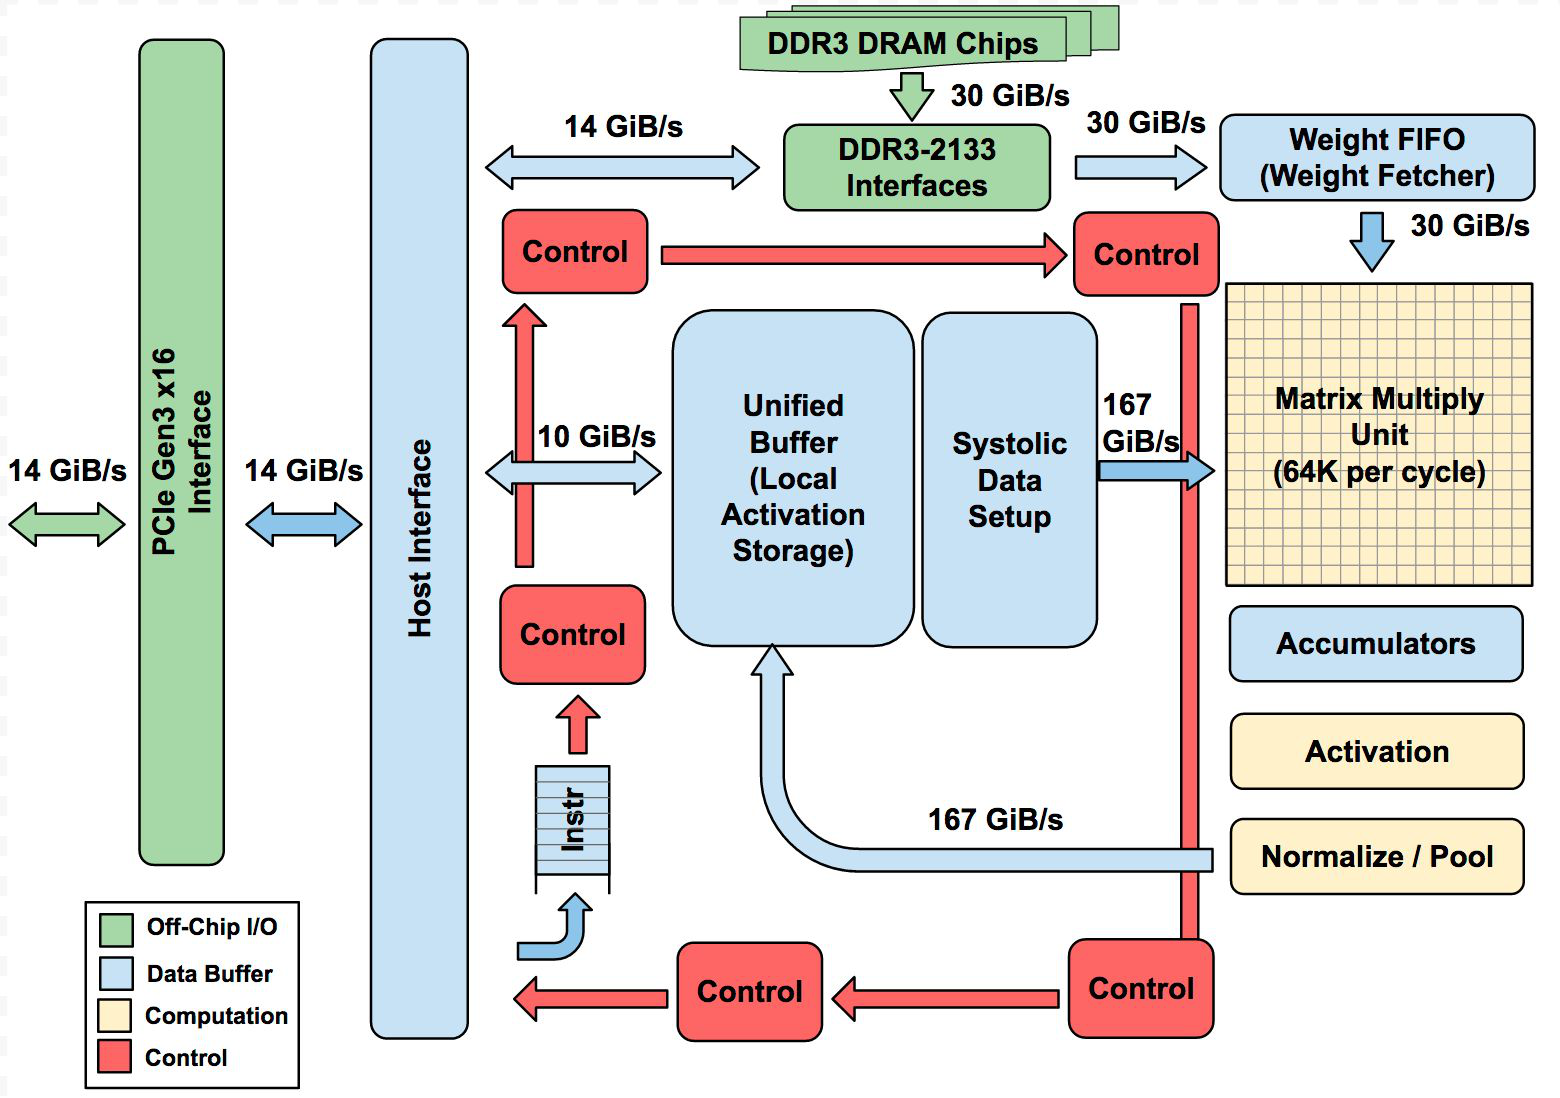
\includegraphics[width=1\textwidth]{tpu.png}
\label{fig:tpu}
\end{figure}

\section{RISC-V}

RISC-V~\cite{risc_v_manual} is an open-source instruction set architecture (ISA) that has recently gained popularity due to its modularity, scalability, and flexibility. Unlike traditional proprietary ISAs, RISC-V is freely available for academic and commercial use and allows users to design custom instruction sets tailored to their specific application requirements. This makes RISC-V attractive for embedded systems, Internet of Things (IoT) devices, and other resource-constrained applications.

The RISC-V ISA is based on a simple load-store architecture that employs a small set of basic instructions that can be combined to perform complex operations. This simplicity allows for a smaller, more power-efficient implementation and easier verification and testing. Moreover, RISC-V supports variable-length instructions, which means it can support different instruction sizes depending on the application requirements.

One of the key advantages of RISC-V is its modularity. The ISA is divided into several standard extensions, such as the Integer, Floating-Point, and Vector extensions, that can be selectively included or excluded depending on the application requirements~\cite {risc_v_manual}. This allows for a highly customizable and scalable implementation optimized for specific use cases. Another advantage of RISC-V is its open-source nature. The ISA is developed and maintained by the RISC-V Foundation, a non-profit organization that promotes the use and adoption of the RISC-V ISA. This open-source model encourages collaboration and innovation, allowing for a more transparent and inclusive development process.

\subsection{Custom Function Unit}

Custom Function Units (CFUs) are specialized hardware that can be integrated into a general-purpose processor to accelerate specific operations or tasks. CFUs are designed to work in tandem with the processor, offloading computation from the main pipeline and reducing the system's overall energy consumption and latency. 

Authors in~\cite{risc_v_cfu} propose the implementation of CFU for RISC-V ISA. CFU is invoked by a custom R-format ISA instruction (Fig.~\ref{fig:r-format}) added to the CPU. R-format instruction has two input registers with the size of 32 bits ($rs1$, $rs2$), a destination register ($rd$), and 10 bits to encode what operation to perform ($funct7$ and $funct3$). 

\begin{figure}[t]
\centering
\caption{RISC-V R instruction format~\cite{risc_v_manual}}
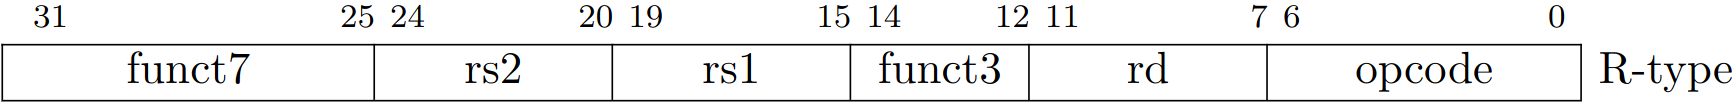
\includegraphics[width=1\textwidth]{r-format.png}
\label{fig:r-format}
\end{figure}

A two-way handshake is used for CPU-to-CFU communication. When the CPU calls CFU, it puts $funct7$, $funct3$, and both operands on the bus. After that, signal $cmd\_valid$ is set to 1 to ask CFU to start the computation. CFU confirms that it received a request by setting $cmd\_ready$ to 1. CPU is stuck until a response is returned. When the job is done, CFU informs CPU by setting $rsp\_ready$ to 1, and CPU acknowledges the response with $rsp\_valid$. The timing diagram is shown in Fig.~\ref{fig:cfu-timing}.

\begin{figure}[t]
\centering
\caption{CFU timing diagram (CFU-L2 signaling protocol)~\cite{risc_v_cfu}}
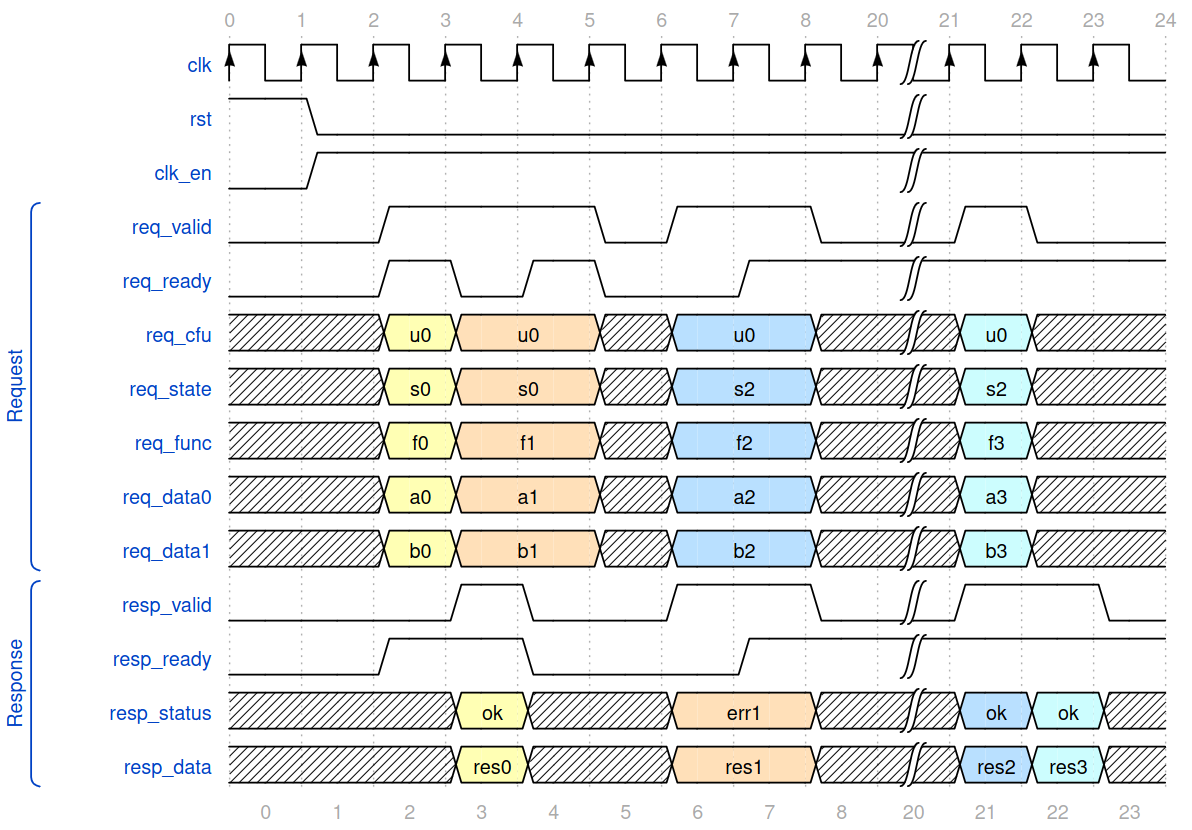
\includegraphics[width=1\textwidth]{cfu-protocol.png}
\label{fig:cfu-timing}
\end{figure}

CFU doesn't impose any restrictions on the hardware design -- the only limiting factor is FPGA resources. But there are two important limitations:
\begin{itemize}
    \item Interface is strictly R-format~\ref{fig:r-format}, and no changes are permitted without direct interference with ISA implementation,
    \item CFU doesn't have access to the RAM of the CPU.
\end{itemize}
Because of the second restriction, the current CFU specification limits the acceleration potential since the CPU has to copy data to the on-chip memory buffer accessible by the accelerator. 

\section{Field Programmable Gate Array}
FPGAs are programmable logic devices that allow digital circuits and systems to be implemented through configurable logic blocks and interconnections. FPGAs offer high flexibility and customization, as they can be reprogrammed to implement different circuits or functions.

FPGAs are typically programmed using a Hardware Description Language (HDL), such as Verilog or VHDL, which describes the functionality and behavior of the circuit to be implemented. The HDL code is then synthesized into a configuration file that can be loaded onto the FPGA, configuring it to implement the desired circuit. 

FPGAs consist of many configurable logic blocks (CLBs), input/output (I/O) blocks, and resources interconnected through a programmable routing matrix. Each CLB typically contains a lookup table (LUT), which can implement any Boolean function, and a flip-flop or latch for storing state. The interconnect resources consist of programmable switches and wires that can be configured to connect the CLBs and I/O blocks as needed. The routing matrix provides a flexible and customizable way to connect the logic blocks and I/O blocks, allowing various circuit topologies and functions to be implemented~\cite{fpga_architecture}.

One of the key benefits of FPGAs is their ability to provide hardware acceleration for computationally intensive tasks. FPGAs can be programmed to implement custom hardware accelerators for specific applications, providing significant speedup and energy efficiency compared to software-based implementations on general-purpose processors.~\cite{cpu_vs_gpu_vs_fpga}

FPGAs also offer other benefits, such as high throughput~\cite{fpga_high_throughput} and integrating multiple functions or peripherals into a single device. Finally, FPGAs are also highly adaptable, allowing for quick iterations and modifications to the design. Experiments are often conducted on the FPGA, and later design is deployed as Application-specific integrated circuit (ASIC)~\cite{fpga_to_asic}. After design finalization, ASIC is synthesized to reduce power consumption and design area and further improve the accelerator's throughput, latency, price, etc~\cite{fpga_vs_asic}. 

Diagram showing high-level architecture of Xilinx FPGA --~Fig.\ref{fig:fpga_diagram}.

\begin{figure}[t]
\centering
\caption{High-level Xilinx FPGA architecture overview. Credit:~\cite{fpga_diagram}}
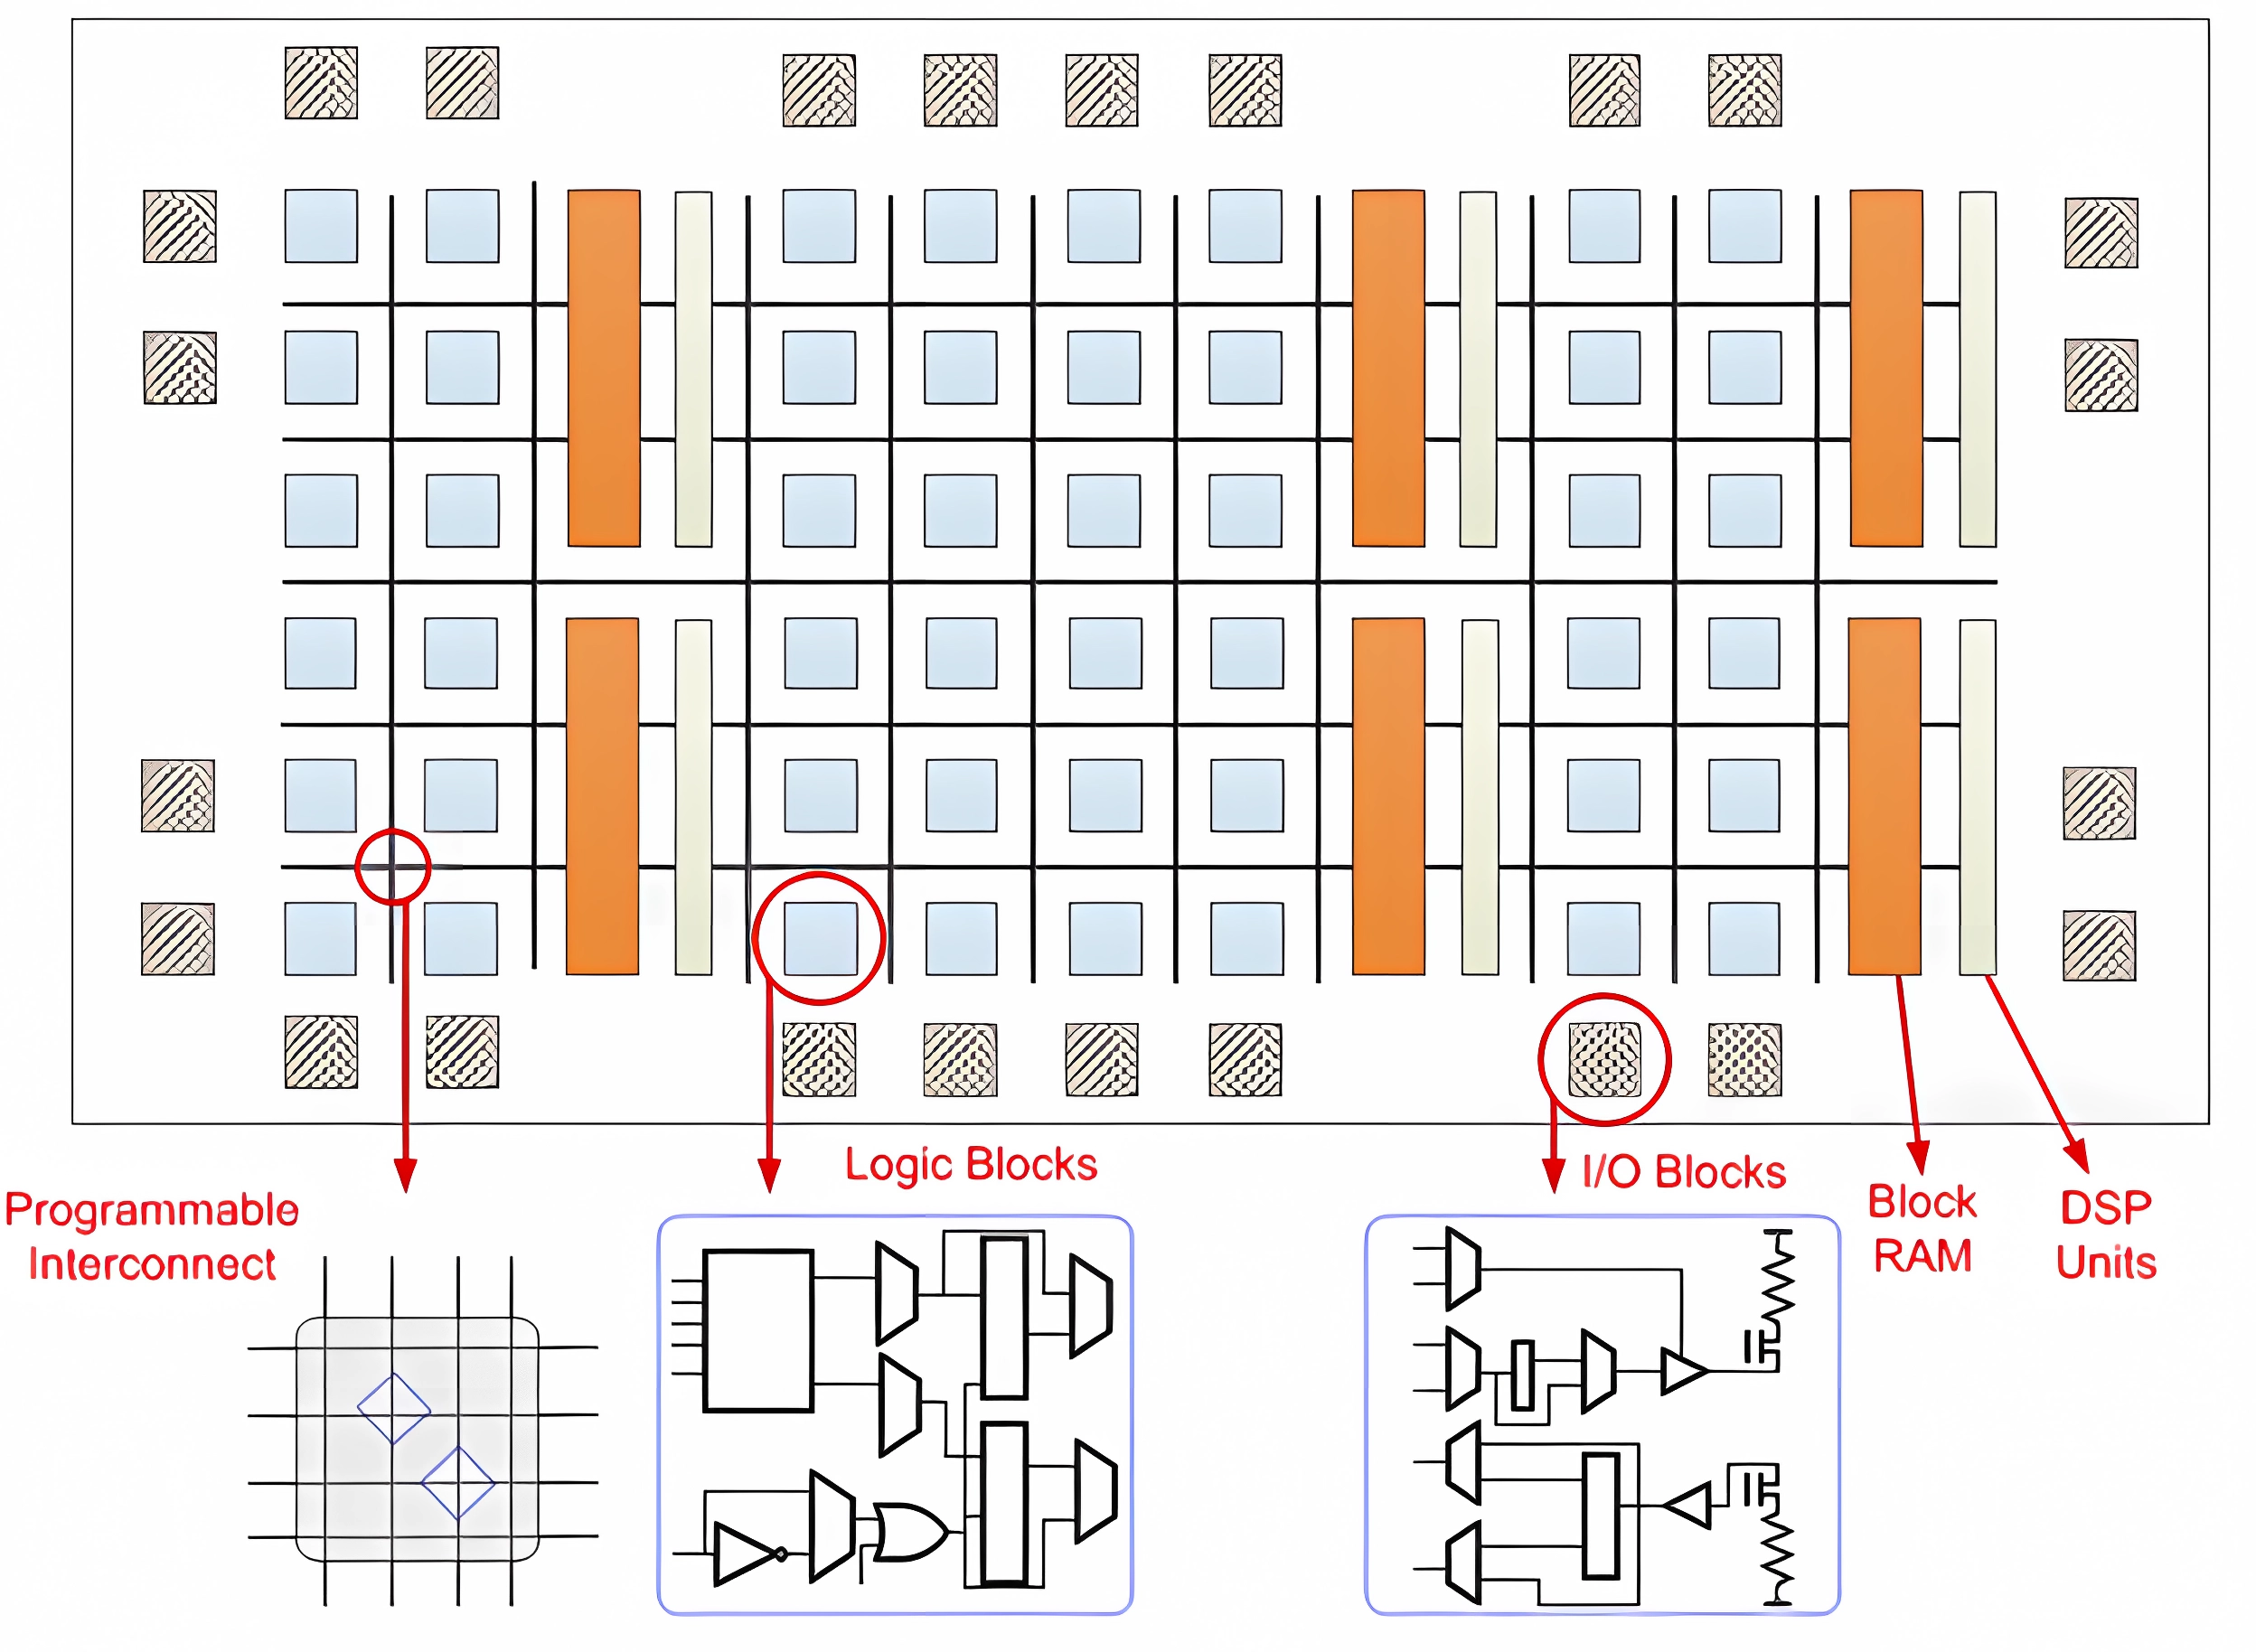
\includegraphics[width=1\textwidth]{graphic/fpga_diagramx4.png}
\label{fig:fpga_diagram}
\end{figure}